\subsection{Initializing}
After the user runs an application, an initialization step should happen to introduce itself to the other applications. This step uses the Device Introduction event. Figure \ref{fig:Initializing} shows a source application that joins the network and introduces itself with a message to library. Library publishes this message to all supported topics of Application State Models, and middleware forwards it to the library of the target application which subscribed to the same topic. Thereby, the library add the new device to a device list and notifies the target application about a new device. In response, target application introduce itself in the same way to the source application.



\FloatBarrier \begin{figure}[H]
    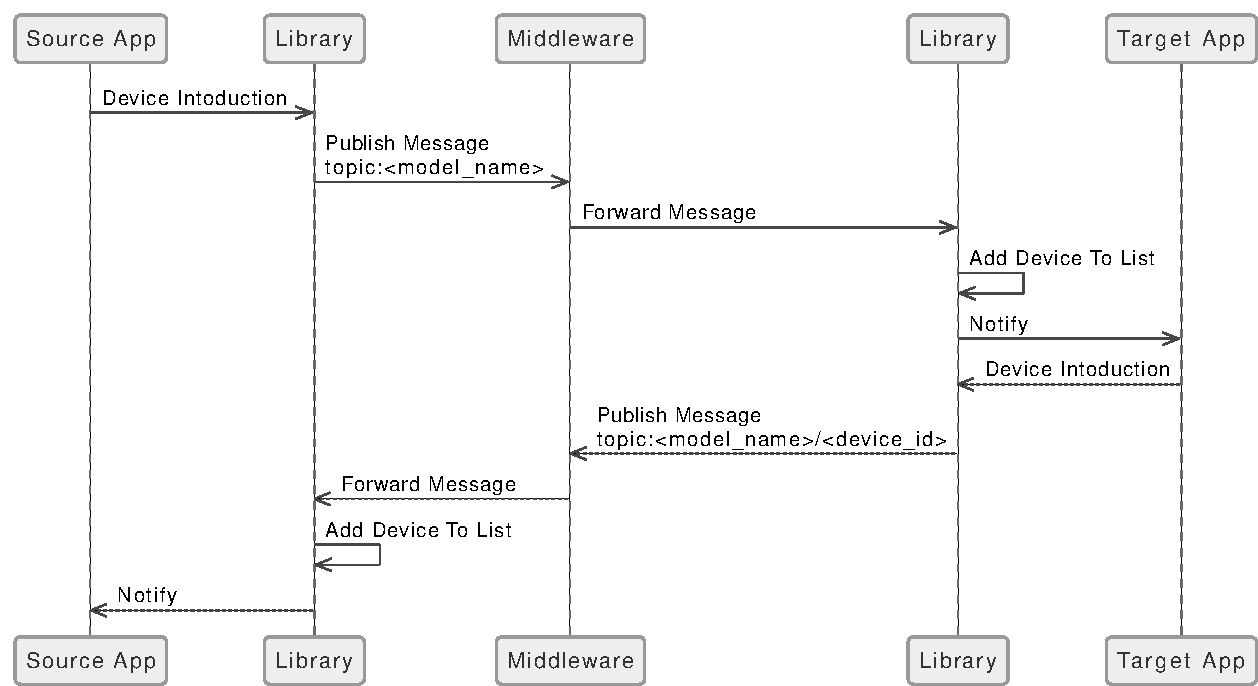
\includegraphics[width=\linewidth]{../figures/Initializing.pdf}
    \centering
    \caption{Initializing the Source Application}
    \label{fig:Initializing}
\end{figure} \FloatBarrier

\subsection{Going Offline}
An application might go offline by a user or even by other causes. A plan should cover these incidents. This step uses the Device Leave event. After disconnection, other devices are not allowed to send any message to that particular device.

\subsubsection{Graceful}
A user might close the application. In this case, the application goes offline gracefully, and it should notify other applications about its absence. Figure \ref{fig:Going-Offline-Graceful-Source} shows the source application going offline gracefully. With the library's help, the source application informs its absence to middleware on \lstinline[basicstyle=\ttfamily]{online} topic, and middleware forwards it to the library of the target application. Thereby, the library removes the device from devices list and notifies the target application about the leaving of the source application. 

\FloatBarrier \begin{figure}[H]
    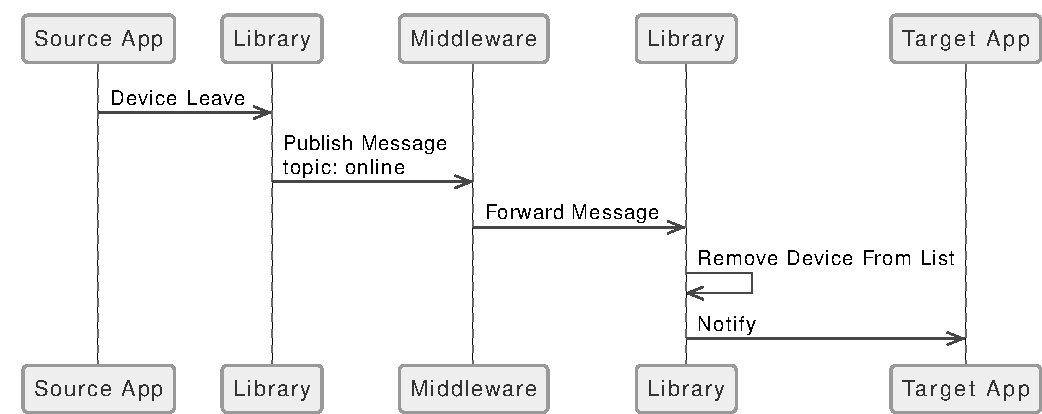
\includegraphics[width=\linewidth]{../figures/Going-Offline-Graceful-Source.pdf}
    \centering
    \caption{Going Offline Gracefully: Source}
    \label{fig:Going-Offline-Graceful-Source}
\end{figure} \FloatBarrier

\subsubsection{Ungraceful}
An application might go offline by other causes like network problems, device crashing, application failure, etc. In this case, the application goes offline ungracefully, and it should notify other applications about its absence. Figure \ref{fig:Going-Offline-Ungraceful-Source} shows the source application going offline ungracefully. The middleware checks if the application is connected; if it does not get any response, request gets a timeout and it publishes a message to  \lstinline[basicstyle=\ttfamily]{online} topic. Thereby, the library removes the device from devices list notifies the target application about the leaving of the source application.

\FloatBarrier \begin{figure}[H]
    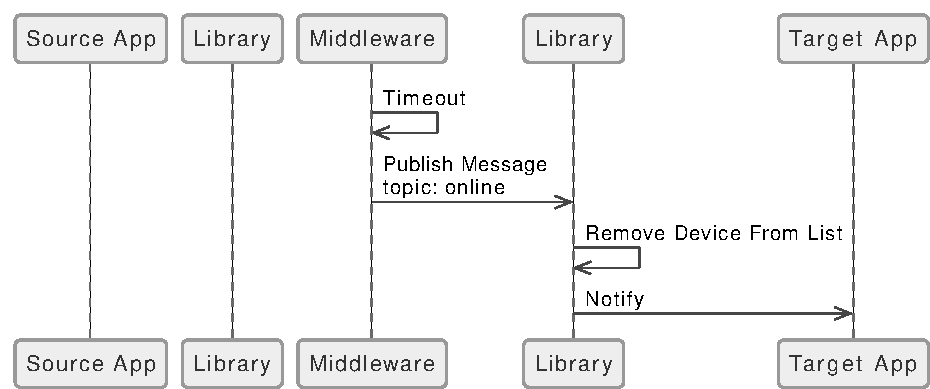
\includegraphics[width=\linewidth]{../figures/Going-Offline-Ungraceful-Source.pdf}
    \centering
    \caption{Going Offline Ungracefully: Source}
    \label{fig:Going-Offline-Ungraceful-Source}
\end{figure} \FloatBarrier

\subsubsection{Has Run-Time State}
To migrate a run-time state, an application should have a run-time state. Any application with a run-time state should notify other applications about it if they request a run-time state. This step uses the Device Has State event. Figure \ref{fig:Inform-Devices-Has-State-Source} shows the source application has a run-time state and informs the middleware by publish a message to topics of Application State Models and middleware forward it to the library of the target application. Thereby, the library notifies the target application about the source application, which has a run-time state.

\FloatBarrier \begin{figure}[H]
    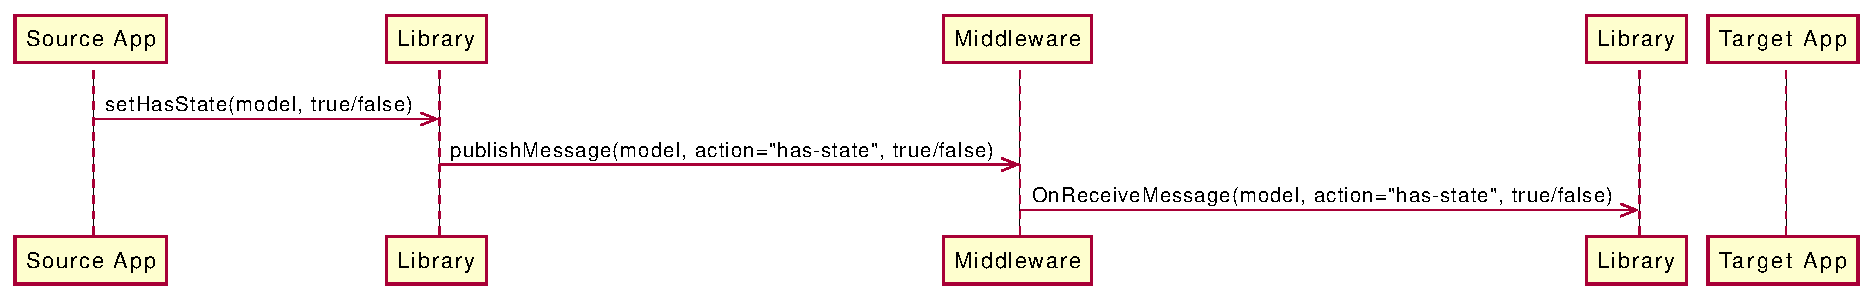
\includegraphics[width=\linewidth]{../figures/Inform-Devices-Has-State-Source.pdf}
    \centering
    \caption{Source App inform other devices that has a state}
    \label{fig:Inform-Devices-Has-State-Source}
\end{figure} \FloatBarrier

\subsection{Store Run-time State}
To migrate a run-time state of an application, it should be temporarily stored and ready for migration if other applications request it. Figure \ref{fig:Store-Current-State} shows that the source and target applications can temporarily store their run-time state in the library.

\FloatBarrier \begin{figure}[H]
    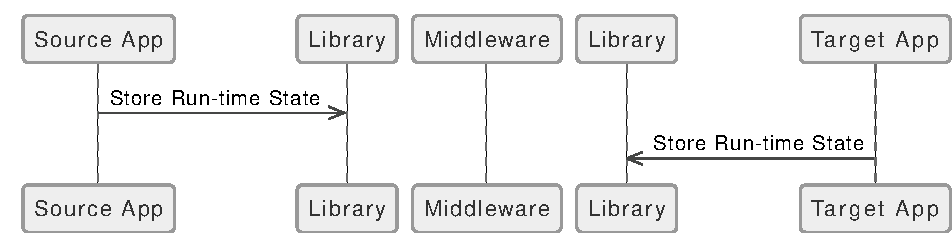
\includegraphics[width=\linewidth]{../figures/Store-Current-State.pdf}
    \centering
    \caption{Store the Current State}
    \label{fig:Store-Current-State}
\end{figure} \FloatBarrier


\subsection{Migration Patterns}
In this section, we describe two patterns for run-time state migration.

\subsubsection{Pull Method}
In the pull method, source applications request a run-time state from the target application. Figure \ref{fig:Migration-Source-to-Target-Pull-Method} shows the source application gets the list of devices with a common Application State Model, then selects the target application and requests its run-time state by sending a message from the library to middleware. The middleware forwards the message, and the target application gets a request of its run-time state. After processing the request, the target application sends its run-time state by the library to middleware. The middleware forwards the message, and the source application receives the run-time state. Source application adjusts the new run-time state and notifies the target application about finalizing the run-time state migration by sending a message to the library and middleware. 

\FloatBarrier \begin{figure}[H]
    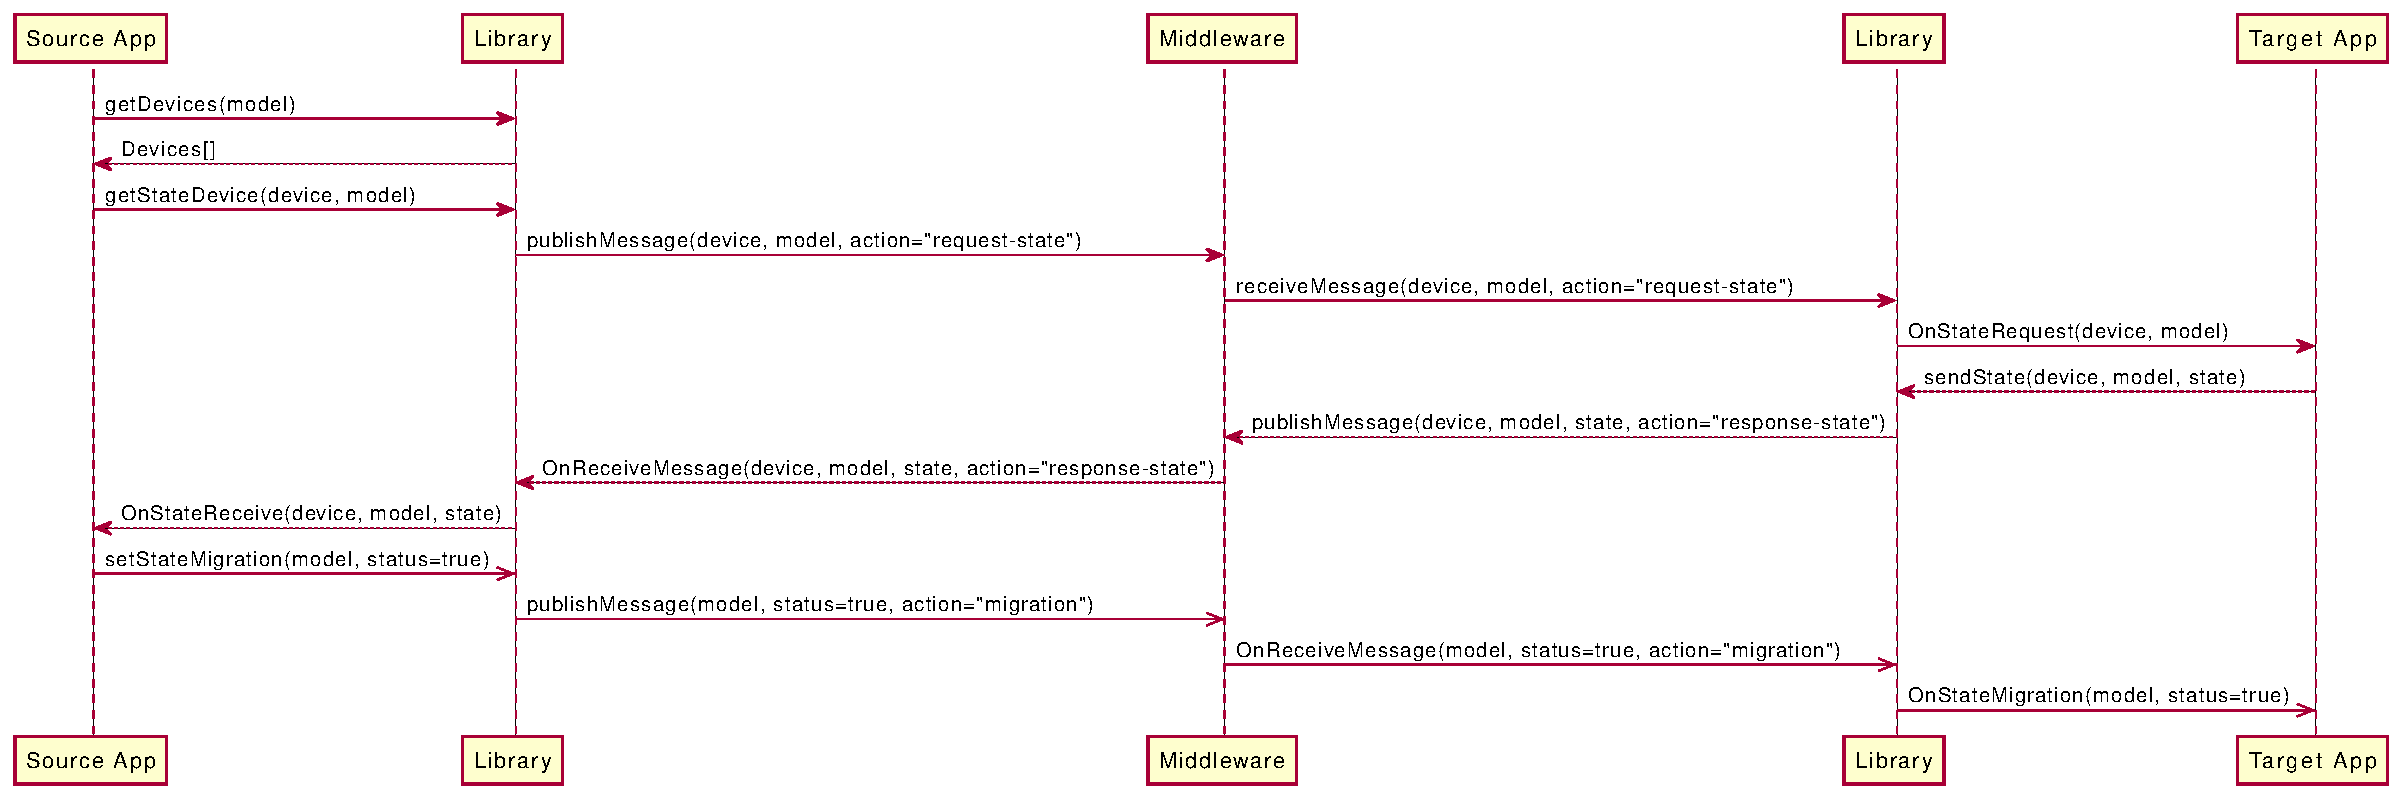
\includegraphics[width=\linewidth]{../figures/Migration-Source-to-Target-Pull-Method.pdf}
    \centering
    \caption{Pull Method: Migration Source to Target}
    \label{fig:Migration-Source-to-Target-Pull-Method}
\end{figure} \FloatBarrier

\subsubsection{Push Method}
In the push method, source applications send their run-time state to the target application without a request by force. Figure \ref{fig:Migration-Source-to-Target-Push-Method} shows the source application gets the list of devices with a common Application State Model, then selects the target application and requests its run-time state by sending a message from the library to middleware. The middleware forwards the message, and the target application gets a request of its state. After processing the request, the target application sends its run-time state by the library to middleware. The middleware forwards the message, and the source application receives the run-time state. Source application adjusts the new run-time state and notifies the target application about finalizing the run-time state migration by sending a message to the library and middleware. 

\FloatBarrier \begin{figure}[H]
    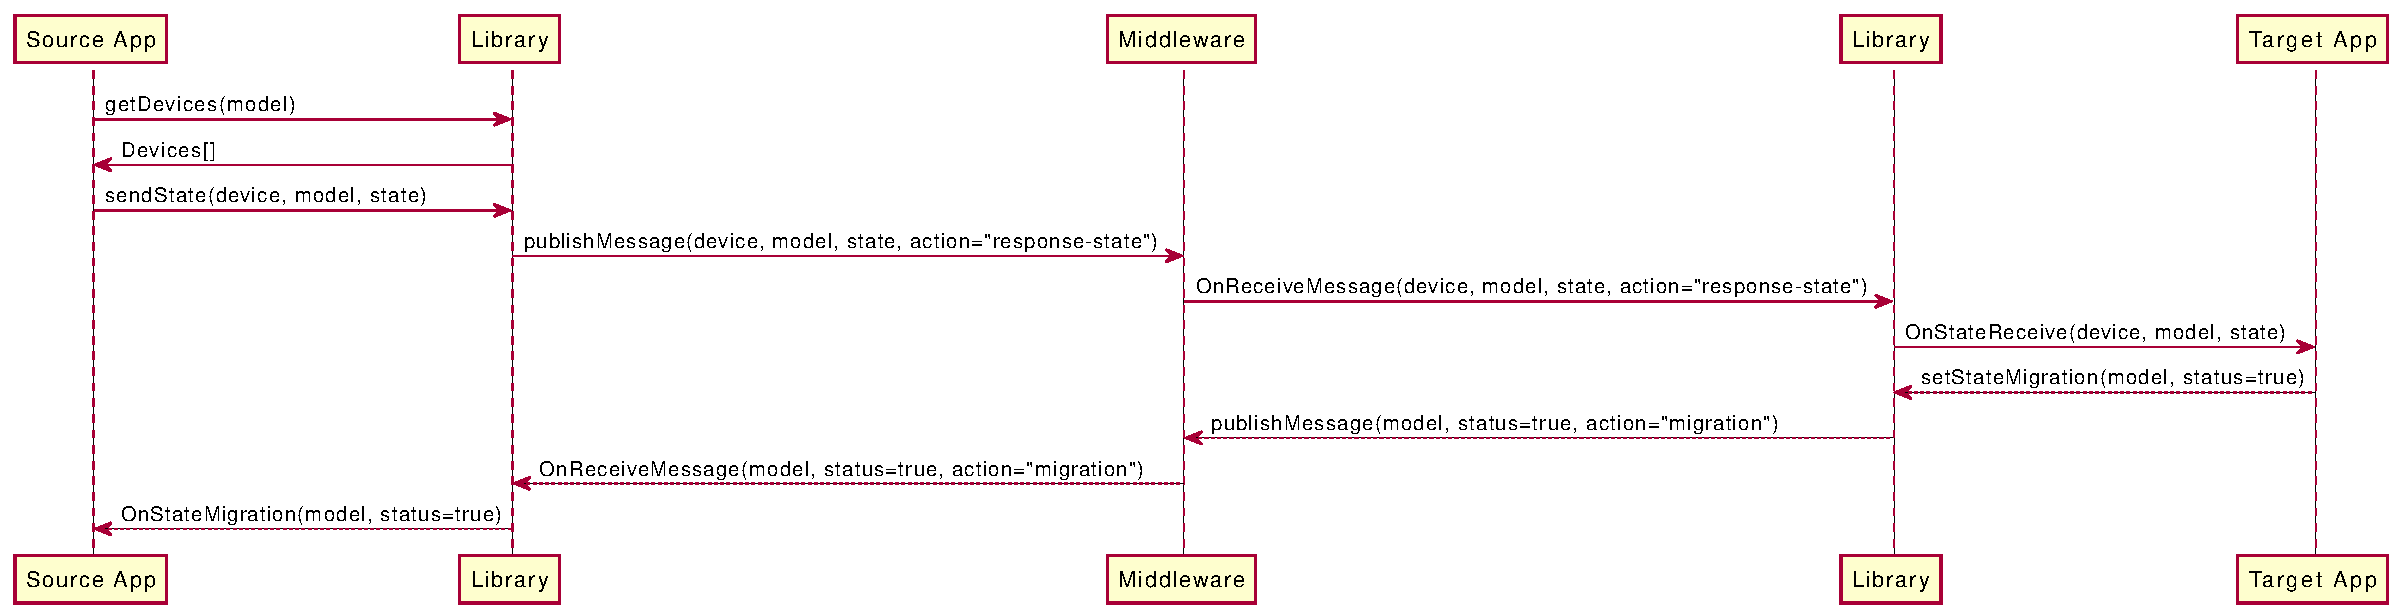
\includegraphics[width=\linewidth]{../figures/Migration-Source-to-Target-Push-Method.pdf}
    \centering
    \caption{Push Method: Migration Source to Target}
    \label{fig:Migration-Source-to-Target-Push-Method}
\end{figure} \FloatBarrier

